\documentclass[11pt,a4paper]{article}
\usepackage[T1]{fontenc}
\usepackage[utf8]{inputenc}
\usepackage[czech]{babel}
\usepackage{lmodern}
\usepackage{geometry}
\geometry{top=27mm,bottom=20mm,left=22mm,right=22mm,headsep=7mm}
\usepackage{amsmath,amssymb,siunitx,graphicx,booktabs,longtable,array,float,caption,microtype,hyperref,xcolor,fancyhdr,enumitem}\hypersetup{hidelinks}
\sisetup{output-decimal-marker={,},exponent-product=\cdot,per-mode=symbol}
\setlength{\parindent}{0pt}
\setlength{\parskip}{4pt}
\captionsetup{font=small,labelfont=bf}
\captionsetup[table]{position=top,skip=6pt}
\captionsetup[figure]{position=bottom,skip=7pt}
\renewcommand{\arraystretch}{1.35}
\setlength{\tabcolsep}{6pt}
\setlength{\arrayrulewidth}{0.45pt}
\pagestyle{fancy}\fancyhf{}
\setlength{\headheight}{25pt}
\newcommand{\labname}{Modelování složek komplexní permitivity}
\fancyhead[L]{\footnotesize Pavel Pernička}
\fancyhead[C]{\footnotesize\bfseries Lab 1}
\fancyhead[R]{\parbox[b]{0.49\textwidth}{\raggedleft\footnotesize Modelování složek komplexní permitivity}}
\fancyfoot[C]{\thepage}
\renewcommand{\headrulewidth}{0.4pt}
\setlist[enumerate]{itemsep=3pt,topsep=3pt}
\begin{document}

\section{Debyeho model komplexní permitivity}
Pro parametry $\varepsilon_s=60$, $\varepsilon_\infty=5$ a
$\tau=3{,}7\cdot10^{-5}\,\mathrm{s}$ vypočteny
závislosti reálné a imaginární složky relativní permitivity a
ztrátového činitele na úhlové frekvenci $\omega=2\pi f$:
\begin{align}
\varepsilon'(\omega)&=\varepsilon_\infty+\frac{\varepsilon_s-\varepsilon_\infty}{1+(\omega\tau)^2},\\
\varepsilon''(\omega)&=\frac{(\varepsilon_s-\varepsilon_\infty)\omega\tau}{1+(\omega\tau)^2},\\
\mathrm{tg}\,\delta(\omega)&=\frac{\varepsilon''(\omega)}{\varepsilon'(\omega)}.
\end{align}

Hodnoty byly zapsány do tabulky a vykresleny v grafu.

\subsection*{Příklad dosazení hodnot}
Pro frekvenci $f=1\,000\,\mathrm{Hz}$ je úhlová frekvence
\begin{equation}
\omega=2\pi f=2\pi\cdot 1\,000
\doteq 6\,283{,}19\,\mathrm{rad\,s^{-1}}.
\end{equation}
Po dosazení parametrů $\varepsilon_s=60$, $\varepsilon_\infty=5$
a $\tau=3{,}7\cdot10^{-5}\,\mathrm{s}$ dostáváme
\begin{align}
\varepsilon' & = 5+\frac{60-5}{1+(6\,283{,}19\cdot 3{,}7\cdot10^{-5})^2}
\doteq 57{,}180,\\[4pt]
\varepsilon'' & = \frac{(60-5)\cdot6\,283{,}19\cdot3{,}7\cdot10^{-5}}{1+(6\,283{,}19\cdot3{,}7\cdot10^{-5})^2}
\doteq 12{,}131,\\[4pt]
\mathrm{tg}\,\delta & =\frac{12{,}13067}{57{,}17989}\doteq 0{,}21215.
\end{align}


\begin{table}[H]
\centering
\caption{Vypočtené hodnoty Debyeho modelu v rozsahu 0 až 1 MHz.}
\label{tab:debye1}
\small
\setlength{\tabcolsep}{6pt}
\renewcommand{\arraystretch}{1.1}
\begin{tabular}{|r|r|r|r|r|}\hline
$f$ [Hz] & $\omega$ [rad/s] & $\varepsilon'$ [--] & $\varepsilon''$ [--] & $\mathrm{tg}\,\delta$ [--] \\ \hline
0 & 0 & 60,000 & 0,000 & 0,00000 \\ \hline
1 & 6,283 & 60,000 & 0,013 & 0,00021 \\ \hline
2 & 12,57 & 60,000 & 0,026 & 0,00043 \\ \hline
5 & 31,42 & 60,000 & 0,064 & 0,00107 \\ \hline
10 & 62,83 & 60,000 & 0,128 & 0,00213 \\ \hline
20 & 125,7 & 59,999 & 0,256 & 0,00426 \\ \hline
50 & 314,2 & 59,993 & 0,639 & 0,01066 \\ \hline
100 & 628,3 & 59,970 & 1,278 & 0,02131 \\ \hline
200 & 1257 & 59,881 & 2,552 & 0,04261 \\ \hline
500 & 3142 & 59,267 & 6,308 & 0,10643 \\ \hline
1\,000 & 6283 & 57,180 & 12,131 & 0,21215 \\ \hline
2\,000 & 1,257e04 & 50,223 & 21,027 & 0,41867 \\ \hline
5\,000 & 3,142e04 & 28,393 & 27,192 & 0,95769 \\ \hline
10\,000 & 6,283e04 & 13,588 & 19,964 & 1,46930 \\ \hline
20\,000 & 1,257e05 & 7,432 & 11,306 & 1,52134 \\ \hline
50\,000 & 3,142e05 & 5,404 & 4,697 & 0,86914 \\ \hline
100\,000 & 6,283e05 & 5,102 & 2,361 & 0,46289 \\ \hline
200\,000 & 1,257e06 & 5,025 & 1,182 & 0,23528 \\ \hline
500\,000 & 3,142e06 & 5,004 & 0,473 & 0,09455 \\ \hline
1\,000\,000 & 6,283e06 & 5,001 & 0,237 & 0,04731 \\ \hline
\end{tabular}
\end{table}
\begin{figure}[H]
\centering
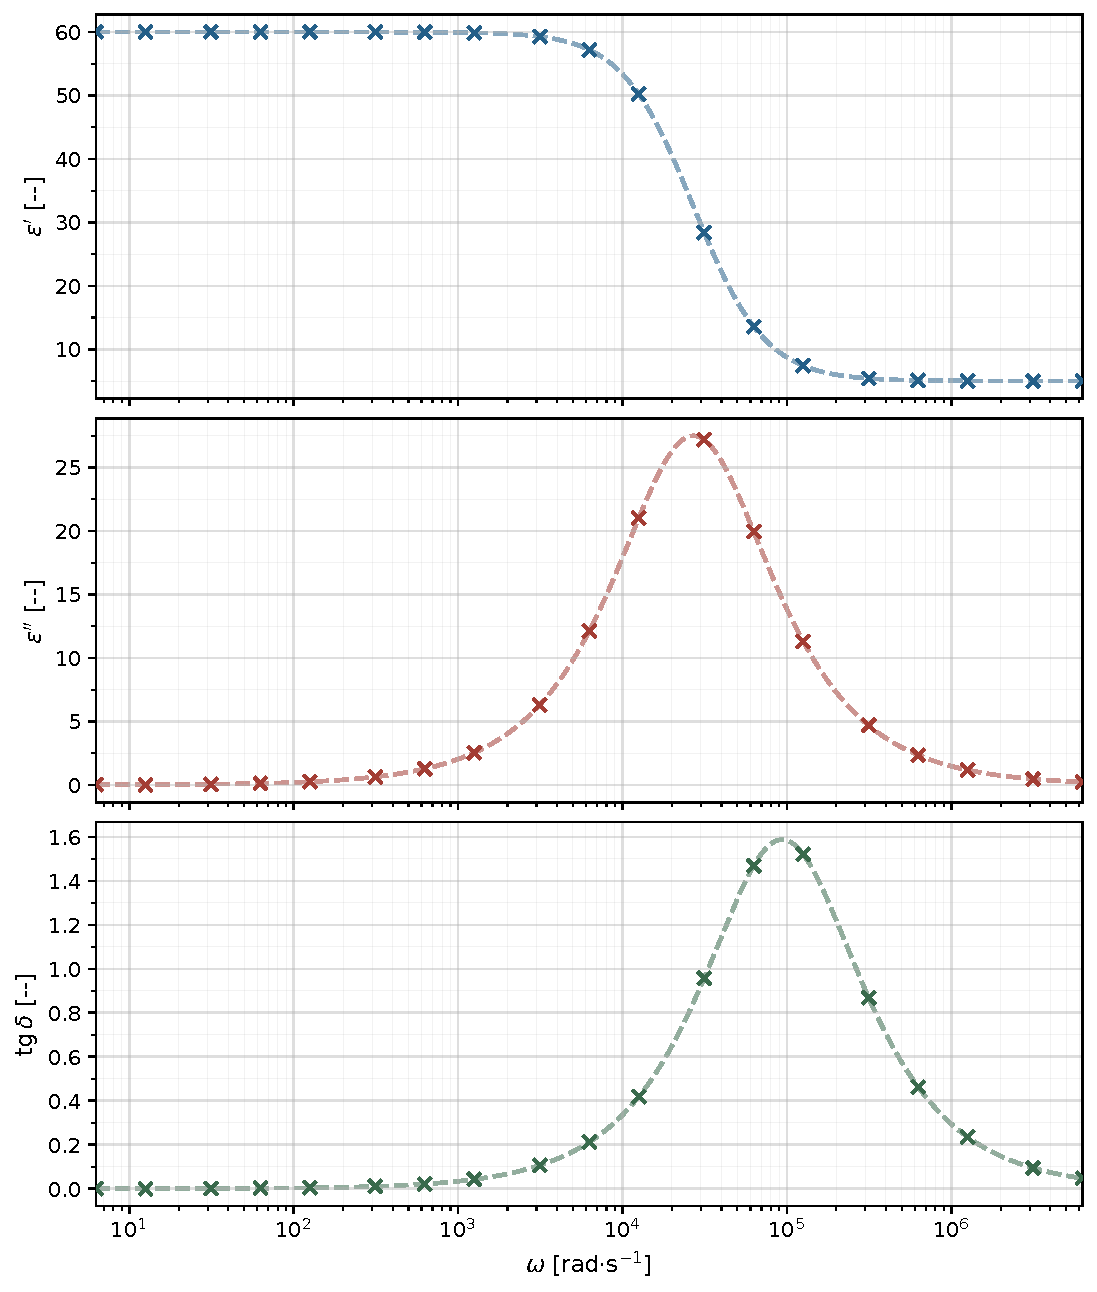
\includegraphics[width=0.90\linewidth]{ukol1_zavislosti.pdf}
\caption{Závislosti $\varepsilon'$, $\varepsilon''$ a $\mathrm{tg}\,\delta$ na úhlové frekvenci $\omega$ podle Debyeho modelu.}
\label{fig:debye1}
\end{figure}


S rostoucí úhlovou frekvencí klesá $\varepsilon'$ od $\varepsilon_s$
k $\varepsilon_\infty$. Imaginární složka $\varepsilon''$ a ztrátový
činitel nejprve rostou k maximu a při vyšších frekvencích klesají.

Stejnou situaci jsme simulovali i v programu Komplexperm, ze kterého jsme získali prakticky identické výstupy:

\begin{figure}[H]
    \centering
    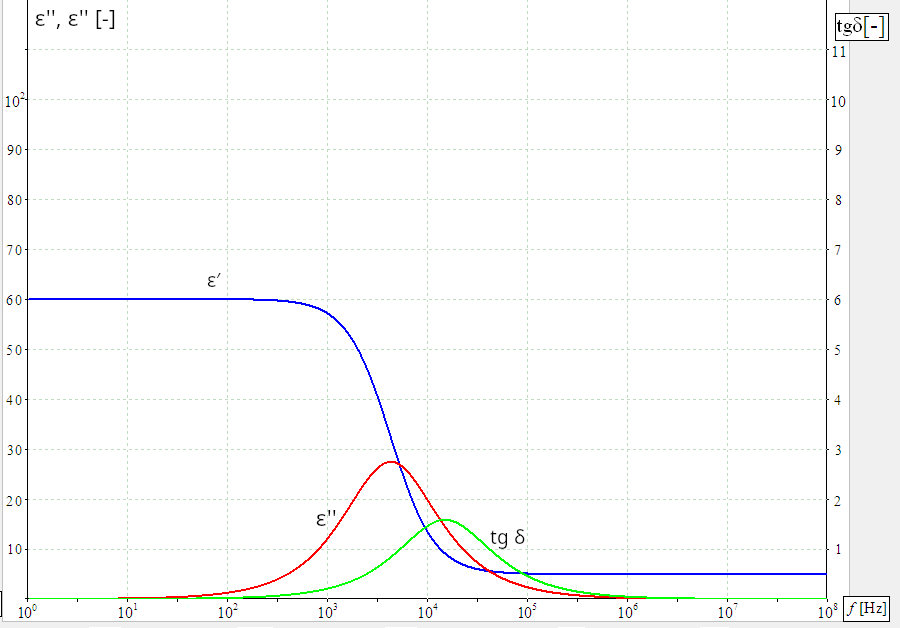
\includegraphics[width=0.7\linewidth]{komplexperm01.png}
    \caption{Frekvenční závislosti reálné a imaginární
    složky permitivity a ztrátového činitele
    simulované v~programu Komplexperm.}
    \label{fig:komplexperm01}
\end{figure}



\section{Modelování podle Cole-Coleho vztahu}

Pomocí programu Komplexperm byly vytvořeny frekvenční
závislosti reálné a imaginární složky permitivity
a ztrátového činitele podle Cole-Coleho vztahu.

\subsection{Vliv distribučního parametru $\alpha$}

Pro simulaci byly použity parametry
\[
\varepsilon_\infty = 2{,}0,\qquad
\varepsilon_s = 8{,}0,\qquad
\tau = 7\cdot10^{-5}\,\mathrm{s},
\]
přičemž distribuční parametr nabýval hodnot
$\alpha = 0;\ 0{,}25;\ 0{,}5$.

\begin{figure}[H]
    \centering
    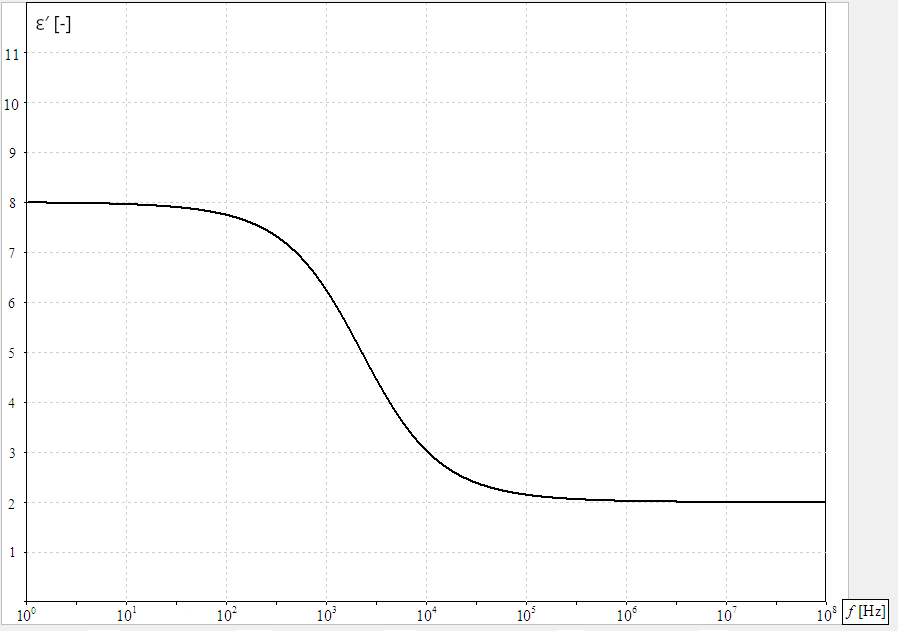
\includegraphics[width=0.7\linewidth]{komplexperm_alpha_tg.png}
    \caption{Závislost reálné složky permitivity
    $\varepsilon'$ na úhlové frekvenci $\omega$
    pro různé hodnoty parametru $\alpha$.}
    \label{fig:alfa-e1}
\end{figure}

\begin{figure}[H]
    \centering
    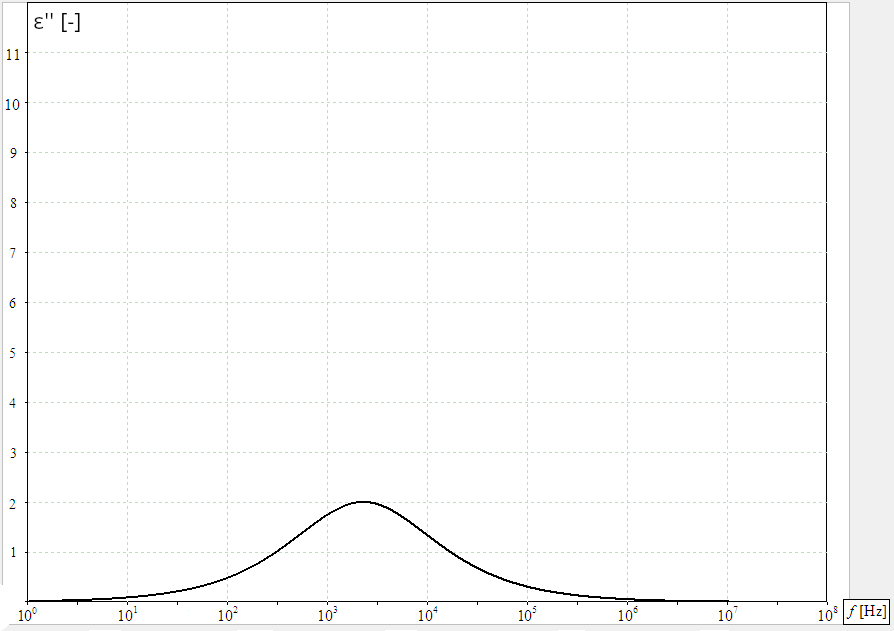
\includegraphics[width=0.7\linewidth]{komplexperm_alpha_e2.png}
    \caption{Závislost imaginární složky permitivity
    $\varepsilon''$ na úhlové frekvenci $\omega$
    pro různé hodnoty parametru $\alpha$.}
    \label{fig:alfa-e2}
\end{figure}

\begin{figure}[H]
    \centering
    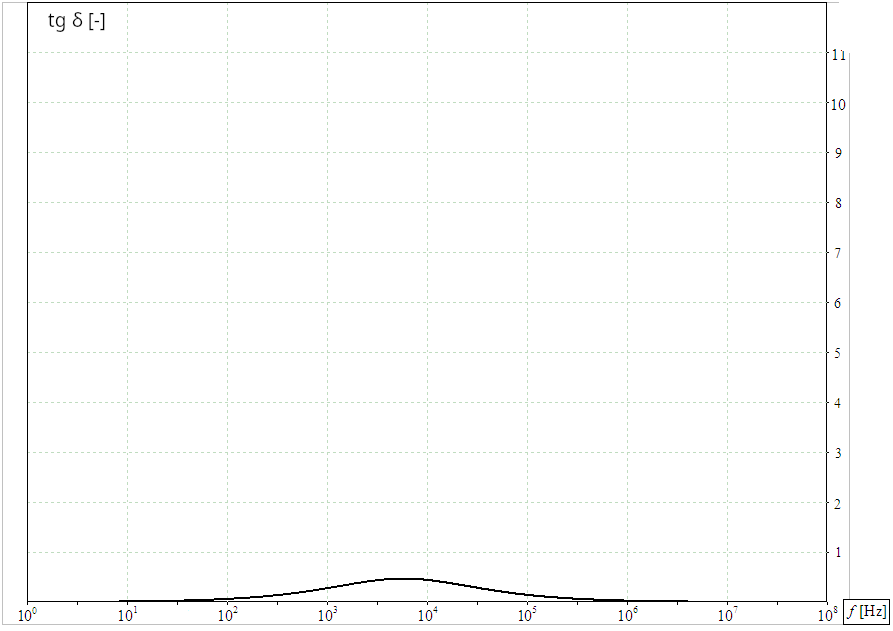
\includegraphics[width=0.7\linewidth]{komplexperm_alpha_e1.png}
    \caption{Závislost ztrátového činitele
    $\mathrm{tg}\,\delta$ na úhlové frekvenci
    $\omega$ pro různé hodnoty parametru $\alpha$.}
    \label{fig:alfa-tg}
\end{figure}

\subsection{Vliv relaxační doby $\tau$}

Pro simulaci byly použity parametry
\[
\varepsilon_\infty = 2{,}0,\qquad
\varepsilon_s = 8{,}0,\qquad
\alpha = 0,
\]
přičemž relaxační doba byla měněna v rozsahu
$\tau = 10^{-4}$ až $5\cdot10^{-7}\,\mathrm{s}$.

\begin{figure}[H]
    \centering
    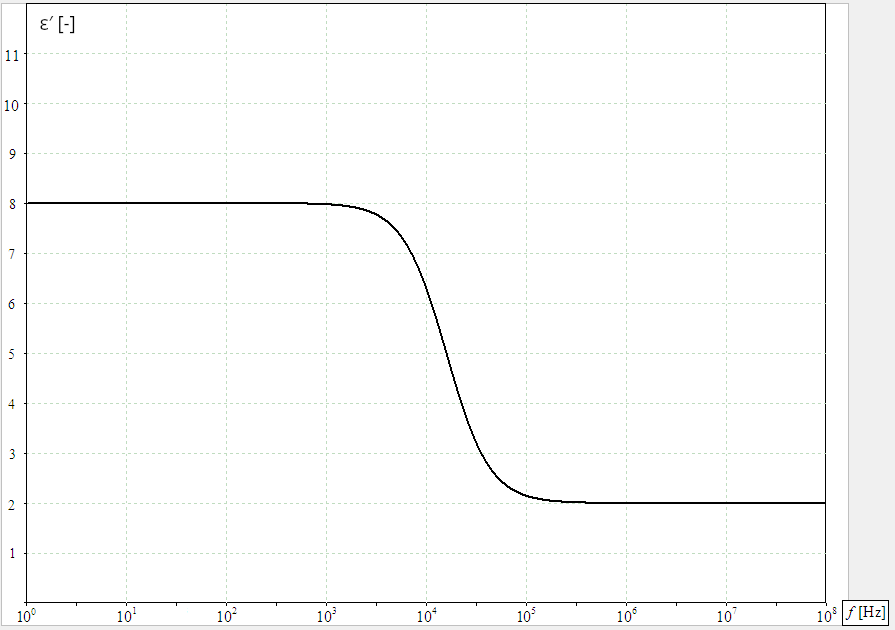
\includegraphics[width=0.7\linewidth]{komplexperm_t_tg.png}
    \caption{Závislost reálné složky permitivity
    $\varepsilon'$ na úhlové frekvenci $\omega$
    pro různé hodnoty relaxační doby $\tau$.}
    \label{fig:tau-e1}
\end{figure}

\begin{figure}[H]
    \centering
    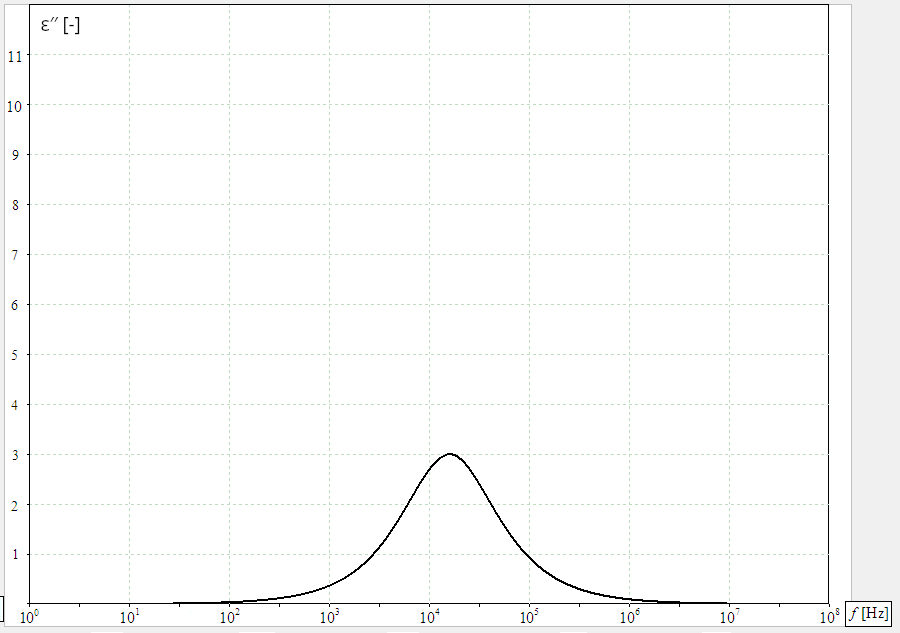
\includegraphics[width=0.7\linewidth]{komplexperm_t_e2.png}
    \caption{Závislost imaginární složky permitivity
    $\varepsilon''$ na úhlové frekvenci $\omega$
    pro různé hodnoty relaxační doby $\tau$.}
    \label{fig:tau-e2}
\end{figure}

\begin{figure}[H]
    \centering
    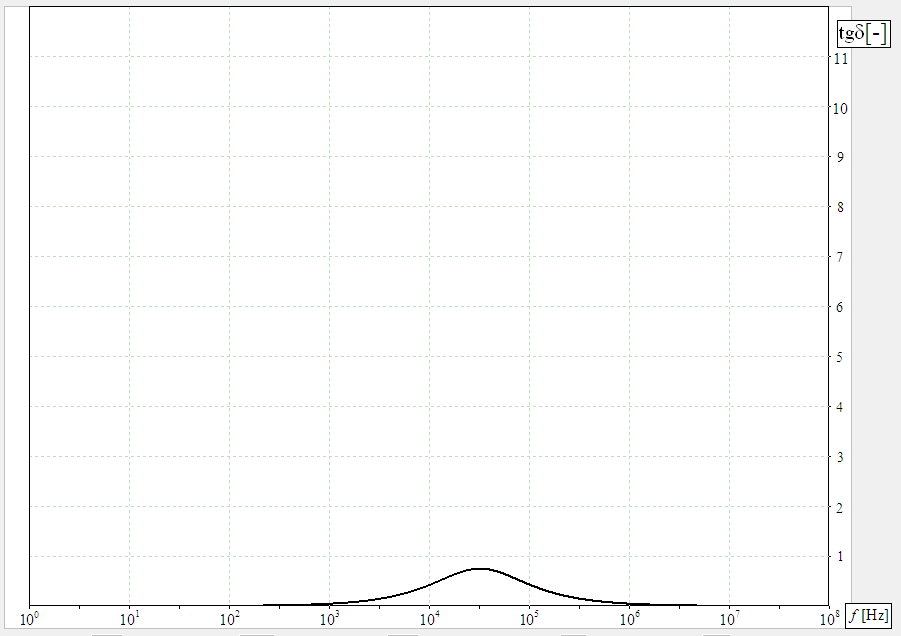
\includegraphics[width=0.7\linewidth]{komplexperm_t_e1.png}
    \caption{Závislost ztrátového činitele
    $\mathrm{tg}\,\delta$ na úhlové frekvenci
    $\omega$ pro různé hodnoty relaxační doby $\tau$.}
    \label{fig:tau-tg}
\end{figure}




\section{Havriliak-Negamiho diagram}

Z Havriliakova-Negamiho diagramu polykarbonátu byl graficky
určen bod, pro který přibližně platí $\omega\tau_0 = 1$
(viz příloha). Tomuto bodu odpovídají hodnoty
$\varepsilon' = 3{,}56$ a $\varepsilon'' = 0{,}075$,
které podle tabulky odpovídají frekvenci přibližně
$f = 180\,\mathrm{Hz}$.

Z této frekvence byla vypočtena střední relaxační doba:
\[
\tau_0 = \frac{1}{\omega}
= \frac{1}{2\pi f}
= \frac{1}{2\pi\cdot180}
\doteq 8{,}84\cdot10^{-4}\,\mathrm{s}.
\]

Po zadání získaných hodnot do programu Diagram byl
vytvořen Havriliakův-Negamiho model s~parametry
\[
\alpha = 0{,}210, \qquad \beta = 0{,}262.
\]

\begin{figure}[H]
    \centering
    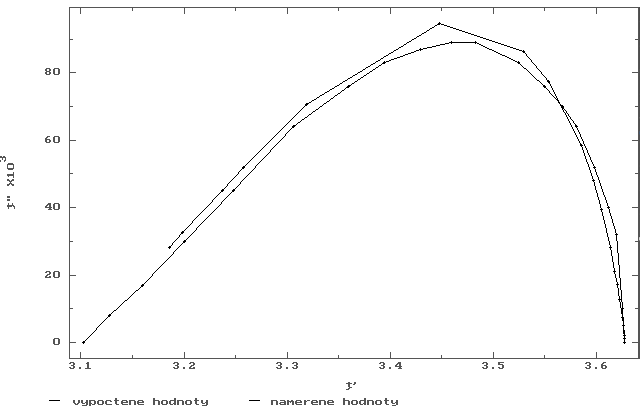
\includegraphics[width=0.7\linewidth]
    {diagram.png}
    \caption{Havriliakův-Negamiho model vytvořený
    programem Diagram.}
    \label{fig:hn-model}
\end{figure}



\section{Manuální výpočet Havriliakova--Negamiho diagramu}

Z parametrů získaných programem Diagram pro polykarbonát
($\alpha=0{,}210$, $\beta=0{,}262$, $\varepsilon_s=3{,}628$,
$\varepsilon_\infty=3{,}102$ a $\tau_0=8{,}4\cdot10^{-4}\,\mathrm{s}$)
jsme vypočítali reálnou a imaginární složku komplexní permitivity
podle Havriliakova--Negamiho vztahu
\begin{equation}
\varepsilon^*(\omega)=\varepsilon_\infty+
\frac{\varepsilon_s-\varepsilon_\infty}
{\left[1+(j\omega\tau_0)^{1-\alpha}\right]^\beta}
=\varepsilon'-j\varepsilon'',\qquad \omega=2\pi f.
\end{equation}

Pro numerický výpočet jednotlivých složek jsme použili vztahy
\begin{align}
r &=\left[1+(\omega\tau_0)^{1-\alpha}
\cos\!\left(\frac{(1-\alpha)\pi}{2}\right)\right]^2
+\left[(\omega\tau_0)^{1-\alpha}
\sin\!\left(\frac{(1-\alpha)\pi}{2}\right)\right]^2,\\
\Theta&=\arctan\!\left(
\frac{(\omega\tau_0)^{1-\alpha}\sin\!\left(\frac{(1-\alpha)\pi}{2}\right)}
{1+(\omega\tau_0)^{1-\alpha}\cos\!\left(\frac{(1-\alpha)\pi}{2}\right)}\right),\\
\varepsilon'&=\varepsilon_\infty+
(\varepsilon_s-\varepsilon_\infty)r^{-\beta/2}\cos(\beta\Theta),\\
\varepsilon''&=(\varepsilon_s-\varepsilon_\infty)r^{-\beta/2}\sin(\beta\Theta).
\end{align}

Příklad dosazení pro $f=1\,000\,\mathrm{Hz}$:
\begin{align*}
\omega&=2\pi\cdot1\,000\doteq6\,283{,}19\,\mathrm{rad\,s^{-1}},\\
r&=\left[1+(6\,283{,}19\cdot8{,}4\cdot10^{-4})^{0{,}790}
\cos\left(\frac{0{,}790\pi}{2}\right)\right]^2\\
&\quad+\left[(6\,283{,}19\cdot8{,}4\cdot10^{-4})^{0{,}790}
\sin\left(\frac{0{,}790\pi}{2}\right)\right]^2
\doteq17{,}26219,\\
\Theta&=\arctan\left(
\frac{(6\,283{,}19\cdot8{,}4\cdot10^{-4})^{0{,}790}
\sin(0{,}790\pi/2)}
{1+(6\,283{,}19\cdot8{,}4\cdot10^{-4})^{0{,}790}
\cos(0{,}790\pi/2)}\right)
\doteq1{,}01120\,\mathrm{rad},\\
\varepsilon'&=3{,}102+(3{,}628-3{,}102)\cdot
17{,}26219^{-0{,}262/2}\cos(0{,}262\cdot1{,}01120)
\doteq3{,}45154,\\
\varepsilon''&=(3{,}628-3{,}102)\cdot
17{,}26219^{-0{,}262/2}\sin(0{,}262\cdot1{,}01120)
\doteq0{,}09484.
\end{align*}

\begin{table}[H]
\centering
\caption{Vypočtené hodnoty složek komplexní permitivity polykarbonátu podle Havriliakova--Negamiho modelu.}
\label{tab:hn-manualni}
\small
\renewcommand{\arraystretch}{1.08}
\begin{tabular}{|r|r|r|}
\hline
$f$ [Hz] & $\varepsilon'$ [--] & $\varepsilon''$ [--] \\ \hline
0 & 3,62800 & -0,00000 \\ \hline
5 & 3,62526 & 0,00720 \\ \hline
10 & 3,62302 & 0,01222 \\ \hline
30 & 3,61456 & 0,02719 \\ \hline
50 & 3,60638 & 0,03819 \\ \hline
100 & 3,58730 & 0,05692 \\ \hline
150 & 3,57055 & 0,06859 \\ \hline
200 & 3,55601 & 0,07633 \\ \hline
300 & 3,53227 & 0,08543 \\ \hline
500 & 3,49875 & 0,09269 \\ \hline
700 & 3,47576 & 0,09474 \\ \hline
1\,000 & 3,45154 & 0,09484 \\ \hline
2\,000 & 3,40686 & 0,09054 \\ \hline
3\,000 & 3,38281 & 0,08632 \\ \hline
10\,000 & 3,32125 & 0,07132 \\ \hline
100\,000 & 3,23818 & 0,04564 \\ \hline
500\,000 & 3,19960 & 0,03285 \\ \hline
1\,000\,000 & 3,18656 & 0,02848 \\ \hline
5\,000\,000 & 3,16260 & 0,02042 \\ \hline
10\,000\,000 & 3,15450 & 0,01769 \\ \hline
\end{tabular}
\end{table}

Vypočtené hodnoty jsme společně s tabulkovými hodnotami polykarbonátu
vynesli do Havriliakova--Negamiho diagramu na obrázku níže.

\begin{figure}[H]
    \centering
    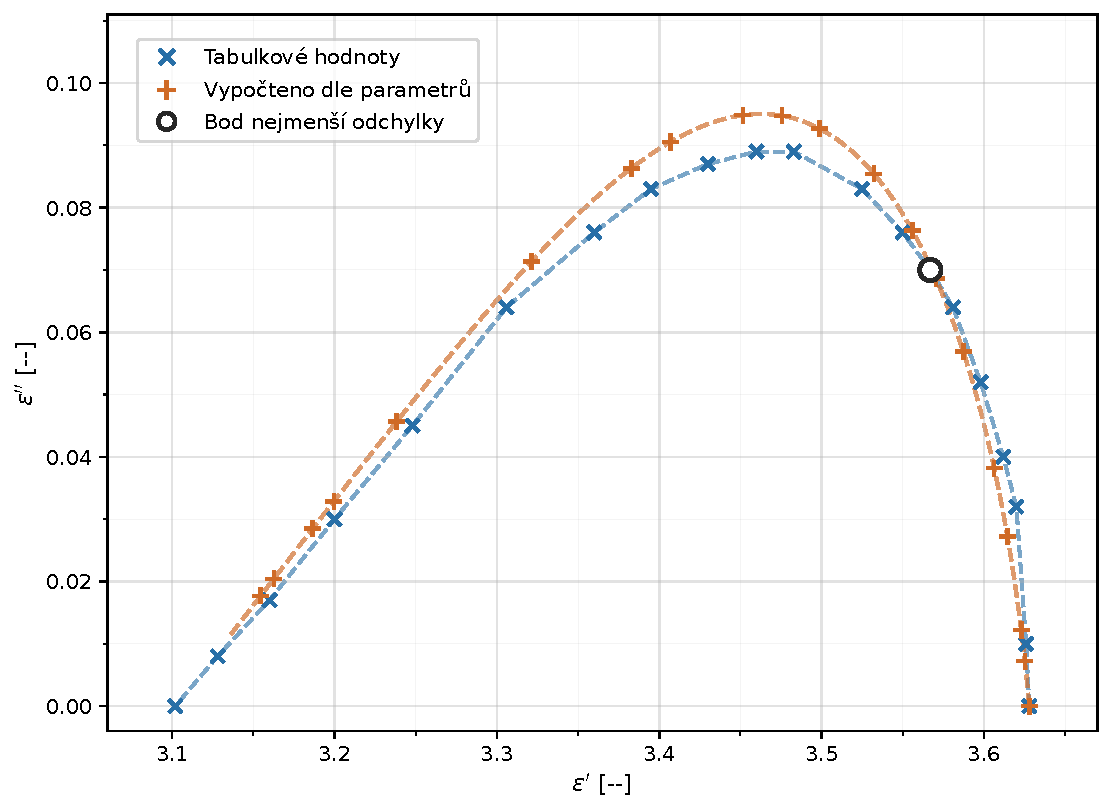
\includegraphics[width=0.90\linewidth]{hn.pdf}
    \caption{Havriliakův--Negamiho diagram porovnávající tabulkové hodnoty polykarbonátu s námi vypočtenýma hodnotama.}
    \label{fig:hn-manualni}
\end{figure}


\section{Závěr}

Pomocí Debyeho rovnic byly vypočteny frekvenční závislosti
reálné a imaginární složky komplexní permitivity a ztrátového
činitele. Vypočtené průběhy odpovídají očekávanému chování
dielektrika. Při nízkých frekvencích se elektrické dipóly
v materiálu stíhají natáčet podle měnícího se elektrického
pole, a proto je relativní permitivita vysoká. S rostoucí
frekvencí však dipóly za změnami pole stále více zaostávají,
což způsobuje pokles reálné složky permitivity $\varepsilon'$
a nárůst ztrát. V oblasti relaxační frekvence
dosahuje imaginární složka permitivity $\varepsilon''$ maxima.

Při ještě vyšších frekvencích se dipóly již nestíhají
dostatečně rychle přorientovávat, jejich příspěvek
k polarizaci klesá a snižují se i ztráty spojené
s tímto mechanismem.

Při modelování Cole-Coleho vztahu bylo zjištěno, že
s rostoucím distribučním parametrem $\alpha$ dochází
k rozšíření relaxační oblasti a snížení maxima
dielektrických ztrát. To odpovídá tomu, že jednotlivé molekuly se přorientovávají různě rychle,
a proto relaxace probíhá v širším rozsahu frekvencí.
Změna relaxační doby $\tau$ naopak způsobuje především
posun frekvenčních závislostí. Při větší relaxační
době reagují dipóly pomaleji a průběhy se posouvají k nižším frekvencím.
Při menší hodnotě $\tau$ se naopak posouvají
k vyšším frekvencím, přičemž jejich tvar
zůstává zachován.

Pro polykarbonát byl z přiloženého Havriliakova--Negamiho diagramu
graficky určen bod, pro který přibližně platí
$\omega\tau_0=1$. Pomocí DOSovského programu Diagram byly
stanoveny distribuční parametry $\alpha=0{,}210$
a $\beta=0{,}262$. Následně byly podle těchto
parametrů manuálně vypočteny složky komplexní
permitivity a porovnány s tabulkovými hodnotami.
Vypočtený průběh poměrně dobře odpovídá tabulkovému a bod nejlepší 
shody se vyskytuje poblíž graficky určeného, pro který platí $\omega\tau_0=1$. 

Ovšem jsou zde patrné menší odchylky, hlavně u vrcholu křivky.
To může být tím, že hodnoty odečtené z grafu nejsou přesné a také tím, 
že pracujeme se zjednodušeným modelem. Reálný materiál se může chovat složitěji.

\end{document}
